\section*{Introduction}

SDSIA is a Python module to generate synthetic data sets for image analysis, and a C library to manipulate these data sets.\\

The goal of the Python module is to provide a way to easily generate data sets of images used by image analysis softwares or algorithms, in a context of learning or development.\\

The generation of the images is made using the 3D rendering software POV-Ray. This software uses text scripts to defined the scene to render, so it's very easy to parameterize a script to create variations of a given scene. The Python module then render as many samples as needed in the set, each time using different parameters' value.\\

By creating its own POV-Ray script, the user can create any needed data set, selecting precisely which aspect of the scene is constant and which is variable. The level of difficulty of the data set, from the point of view of the software or algorithm used for analysis, can then be controlled at will. By choosing the appropriate variable in the scene, the user could also study a particular property of a given software or algorithm (e.g, is it more sensitive to variation in shape or variation in color).\\

Once the user has written the script to render images, the python module takes care of the tedious tasks of rendering (only needed data sets), files and folders management, creation of a description file in JSON format for later use. It also generates perfect masks (black and white image) by modifying the texture properties of the objects in the scene.\\

The number of images per data set, the dimensions and format of each image are also defined by the user. Then, one can create sets corresponding to its needs, in particular memory, disk storage, processing time limits.\\

The current version of SDSIA is designed for image segmentation (localization of pixels corresponding to an object in a scene). However it has been developped with the view to be extended to other kind of data sets.\\

The C library offers the following functionalities: loading a data set from its description file, spitting the data set into user defined categories (e.g. training, validation, test), shuffling the data set, looping through the samples of the data set. It provides the samples of the data set as GenBrush objects to manipulate them easily through this library's functionalities.\\

The C library uses the \begin{ttfamily}PBErr\end{ttfamily}, \begin{ttfamily}GSet\end{ttfamily}, \begin{ttfamily}PBJson\end{ttfamily}, \begin{ttfamily}GenBrush\end{ttfamily} and \begin{ttfamily}PBFileSys\end{ttfamily} libraries.\\

\section{Python module}

\subsection{Usage}

\subsubsection{Unit test}

One can run the unit test with the command python generateDataSet.py. Upon success the following messages will be displayed:

\begin{scriptsize}
\begin{ttfamily}
\verbatiminput{../unitTestPythonRef.txt}
\end{ttfamily}
\end{scriptsize}

If the unit test fails, make sure POV-Ray is correctly installed by running, for example, the comand \begin{ttfamily}./install test\end{ttfamily} in the folder where POV-Ray has been installed (Refer to the POV-Ray documentation for more details). If POV-Ray is correctly installed and the unit test still fails, please contact the developper.

\subsubsection{Create a new data set}

To create a new data set, one has to create the description file and the POV-Ray script for this new data set. Templates for each of them are given below.\\
 
Template for the description file:\\
\begin{scriptsize}
\begin{ttfamily}
\verbatiminput{../dataset.json}
\end{ttfamily}
\end{scriptsize}

DataSetType is a place holder for future version and should always be set to 0. Desc is the description of the data set. Dim are the dimensions of the images (width, height). Supported formats are currently "tga" and "png". NbImg is the number of images to be generated.\\

Template for the POV-Ray script:\\
\begin{scriptsize}
\begin{ttfamily}
\verbatiminput{../dataset.pov}
\end{ttfamily}
\end{scriptsize}

These files must be saved with names, respectively, \begin{ttfamily}dataset-XXX-YYY.json\end{ttfamily} and \begin{ttfamily}dataset-XXX-YYY.pov\end{ttfamily}, where \begin{ttfamily}XXX\end{ttfamily} is the data set group and \begin{ttfamily}YYY\end{ttfamily} is the data set subgroup. One is free to save them wherever she wants but they must be in the same directory. Furthermore, if saved in the POV folders of the SDSIA repository, the module will detect them automatically and one won't need to specify the location of these files with the \begin{ttfamily}-in\end{ttfamily} option.\\

About the POV-Ray script: one must be careful to craft it in such a way that the sequence of random values is the same in both version (image and mask) of the rendering. For example,
\begin{scriptsize}
\begin{ttfamily}
\begin{verbatim}
#if (Mask = 0)
  background { color rgb <rnd(0.0, 1.0), rnd(0.0, 1.0), rnd(0.0, 1.0)> }
#else
  background { color White }
#end

#declare Target = box {
  -1, 1
  scale rnd(0.5, 1.5)
  #if (Mask = 0)
    pigment { color rgb <rnd(0.0, 1.0), rnd(0.0, 1.0), rnd(0.0, 1.0)> }
  #else
    texture {_texMaskTarget}
  #end
}
\end{verbatim}
\end{ttfamily}
\end{scriptsize}
won't render the correct mask. The call to the random generator in the background color being skipped when rendering the mask, the call to the random generator for the scale of the box will return different values. A correct script would be:
\begin{scriptsize}
\begin{ttfamily}
\begin{verbatim}
#declare bgColor = <rnd(0.0, 1.0), rnd(0.0, 1.0), rnd(0.0, 1.0)>;
#if (Mask = 0)
  background { color rgb bgColor }
#else
  background { color White }
#end

#declare Target = box {
  -1, 1
  scale rnd(0.5, 1.5)
  #if (Mask = 0)
    pigment { color rgb <rnd(0.0, 1.0), rnd(0.0, 1.0), rnd(0.0, 1.0)> }
  #else
    texture {_texMaskTarget}
  #end
}
\end{verbatim}
\end{ttfamily}
\end{scriptsize}

\subsubsection{Generate one or several data sets}

One can generate the data sets in the default \begin{ttfamily}POV\end{ttfamily} folder of the SDSIA repository with the command \begin{ttfamily}python generateDataSet.py\end{ttfamily}. One can also specify another folder or one single data set with the \begin{ttfamily}-in\end{ttfamily} argument: \begin{ttfamily}python generateDataSet.py -in <path>\end{ttfamily} where path is the path to the folder containing the data sets' description file and POV-Ray script, or the path to the data set's POV-Ray script.\\

The data sets are generated by default into the DataSets folder of the SDSIA repository, but one can specify another folder with the \begin{ttfamily}-out\end{ttfamily} argument: \begin{ttfamily}python generateDataSet.py -out <path>\end{ttfamily} . Inside the DataSets folder each data set is generated in its own folder as follow: \begin{ttfamily}DataSets/XXX/YYY/\end{ttfamily} where \begin{ttfamily}XXX\end{ttfamily} is the data set group and \begin{ttfamily}YYY\end{ttfamily} is the data set subgroup. Each data set's folder contains one description file (\begin{ttfamily}dataset.json\end{ttfamily}) and the images and masks of the data set. Example of description file:\\
\begin{scriptsize}
\begin{ttfamily}
\verbatiminput{../UnitTestOut/001/001/dataset.json}
\end{ttfamily}
\end{scriptsize}

By default, data sets are only generated if necessary, i.e. the description file and POV-Ray scripts in the input folder are older than the description file in the output folder. One can override this with the argument \begin{ttfamily}-force\end{ttfamily}.\\

One can use the \begin{ttfamily}-simul\end{ttfamily} argument to check what will be generated without actually rendering the images and masks, which may be useful to check that everything will be as expected before running a time consuming generation.\\

\subsubsection{Listing of the data sets}

One can get a listing of the data sets with the command \begin{ttfamily}python generateDataSet.py -list\end{ttfamily}. Example of output:\\
\begin{scriptsize}
\begin{ttfamily}
\verbatiminput{../listing.txt}
\end{ttfamily}
\end{scriptsize}

The listing is generated according to the arguments \begin{ttfamily}-in\end{ttfamily} and \begin{ttfamily}-out\end{ttfamily}.\\

The mark \begin{ttfamily}[*]\end{ttfamily} means the data sets has been generated, and the mark \begin{ttfamily}[ ]\end{ttfamily} means it is not yet generated.

\subsection{Code}

\subsubsection{generateDataSet.py}

\begin{scriptsize}
\begin{ttfamily}
\verbatiminput{../generateDataSet.py}
\end{ttfamily}
\end{scriptsize}

\subsection{exampleUse.py}

A boilerplate to use the generated data sets is given below:
 
\begin{scriptsize}
\begin{ttfamily}
\verbatiminput{../exampleUse.py}
\end{ttfamily}
\end{scriptsize}

\section{C Library}

\subsection{Interface}

\begin{scriptsize}
\begin{ttfamily}
\verbatiminput{/home/bayashi/GitHub/SDSIA/sdsia.h}
\end{ttfamily}
\end{scriptsize}

\subsection{Code}

\subsubsection{sdsia.c}

\begin{scriptsize}
\begin{ttfamily}
\verbatiminput{/home/bayashi/GitHub/SDSIA/sdsia.c}
\end{ttfamily}
\end{scriptsize}

\subsubsection{sdsia-inline.c}

\begin{scriptsize}
\begin{ttfamily}
\verbatiminput{/home/bayashi/GitHub/SDSIA/sdsia-inline.c}
\end{ttfamily}
\end{scriptsize}

\subsection{Unit test}

\begin{scriptsize}
\begin{ttfamily}
\verbatiminput{../unitTestRef.txt}
\end{ttfamily}
\end{scriptsize}

\section{Makefile}

\begin{scriptsize}
\begin{ttfamily}
\verbatiminput{../Makefile}
\end{ttfamily}
\end{scriptsize}

\section{Data sets}

The repository contains several already generated data sets to be used immediately or as references and examples to make new ones.

\subsection{dataset-001-001}

dataset-001-001.json:
\begin{scriptsize}
\begin{ttfamily}
\verbatiminput{../POV/dataset-001-001.json}
\end{ttfamily}
\end{scriptsize}

Example of image and its mask:
\begin{center}
\begin{figure}[H]
\centering
\includegraphics[width=3cm]{./img-001-001.png}
\centering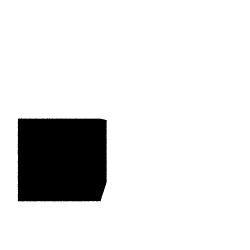
\includegraphics[width=3cm]{./mask-001-001.png}
\end{figure}
\end{center}

dataset-001-001.pov:
\begin{scriptsize}
\begin{ttfamily}
\verbatiminput{../POV/dataset-001-001.pov}
\end{ttfamily}
\end{scriptsize}

\subsection{dataset-001-002}

dataset-001-002.json:
\begin{scriptsize}
\begin{ttfamily}
\verbatiminput{../POV/dataset-001-002.json}
\end{ttfamily}
\end{scriptsize}

Example of image and its mask:
\begin{center}
\begin{figure}[H]
\centering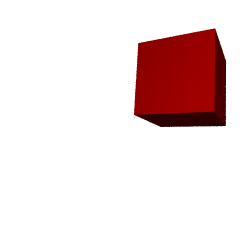
\includegraphics[width=3cm]{./img-001-002.png}
\centering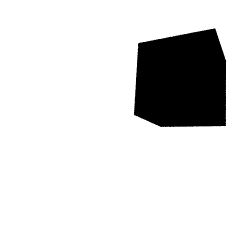
\includegraphics[width=3cm]{./mask-001-002.png}
\end{figure}
\end{center}

dataset-001-002.pov:
\begin{scriptsize}
\begin{ttfamily}
\verbatiminput{../POV/dataset-001-002.pov}
\end{ttfamily}
\end{scriptsize}

\subsection{dataset-001-003}

dataset-001-003.json:
\begin{scriptsize}
\begin{ttfamily}
\verbatiminput{../POV/dataset-001-003.json}
\end{ttfamily}
\end{scriptsize}

Example of image and its mask:
\begin{center}
\begin{figure}[H]
\centering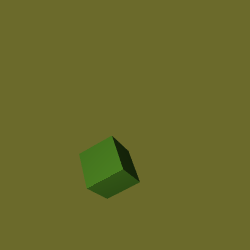
\includegraphics[width=3cm]{./img-001-003.png}
\centering
\includegraphics[width=3cm]{./mask-001-003.png}
\end{figure}
\end{center}

dataset-001-003.pov:
\begin{scriptsize}
\begin{ttfamily}
\verbatiminput{../POV/dataset-001-003.pov}
\end{ttfamily}
\end{scriptsize}

\subsection{dataset-001-004}

dataset-001-004.json:
\begin{scriptsize}
\begin{ttfamily}
\verbatiminput{../POV/dataset-001-004.json}
\end{ttfamily}
\end{scriptsize}

Example of image and its mask:
\begin{center}
\begin{figure}[H]
\centering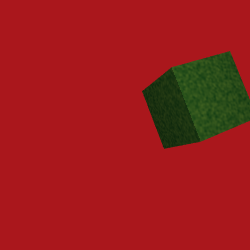
\includegraphics[width=3cm]{./img-001-004.png}
\centering
\includegraphics[width=3cm]{./mask-001-004.png}
\end{figure}
\end{center}

dataset-001-004.pov:
\begin{scriptsize}
\begin{ttfamily}
\verbatiminput{../POV/dataset-001-004.pov}
\end{ttfamily}
\end{scriptsize}

\subsection{dataset-002-001}

dataset-002-001.json:
\begin{scriptsize}
\begin{ttfamily}
\verbatiminput{../POV/dataset-002-001.json}
\end{ttfamily}
\end{scriptsize}

Example of image and its mask:
\begin{center}
\begin{figure}[H]
\centering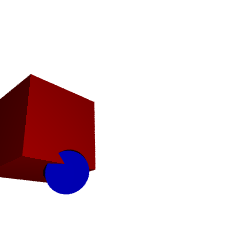
\includegraphics[width=3cm]{./img-002-001.png}
\centering
\includegraphics[width=3cm]{./mask-002-001.png}
\end{figure}
\end{center}

dataset-002-001.pov:
\begin{scriptsize}
\begin{ttfamily}
\verbatiminput{../POV/dataset-002-001.pov}
\end{ttfamily}
\end{scriptsize}

\subsection{dataset-002-002}

dataset-002-002.json:
\begin{scriptsize}
\begin{ttfamily}
\verbatiminput{../POV/dataset-002-002.json}
\end{ttfamily}
\end{scriptsize}

Example of image and its mask:
\begin{center}
\begin{figure}[H]
\centering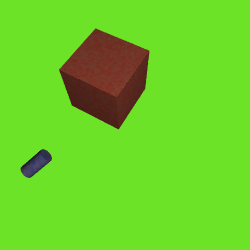
\includegraphics[width=3cm]{./img-002-002.png}
\centering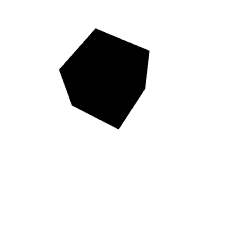
\includegraphics[width=3cm]{./mask-002-002.png}
\end{figure}
\end{center}

dataset-002-002.pov:
\begin{scriptsize}
\begin{ttfamily}
\verbatiminput{../POV/dataset-002-002.pov}
\end{ttfamily}
\end{scriptsize}

\subsection{dataset-002-003}

dataset-002-003.json:
\begin{scriptsize}
\begin{ttfamily}
\verbatiminput{../POV/dataset-002-003.json}
\end{ttfamily}
\end{scriptsize}

Example of image and its mask:
\begin{center}
\begin{figure}[H]
\centering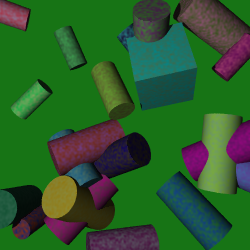
\includegraphics[width=3cm]{./img-002-003.png}
\centering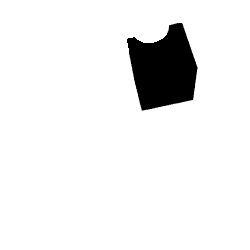
\includegraphics[width=3cm]{./mask-002-003.png}
\end{figure}
\end{center}

dataset-002-003.pov:
\begin{scriptsize}
\begin{ttfamily}
\verbatiminput{../POV/dataset-002-003.pov}
\end{ttfamily}
\end{scriptsize}

